\chapter{Steady-state Phase Space}
\label{apndx:phasespace}
\hspace{\parindent} Shown are the phase space plots for various $b$ values.
\begin{figure}[h!]
 \centering
  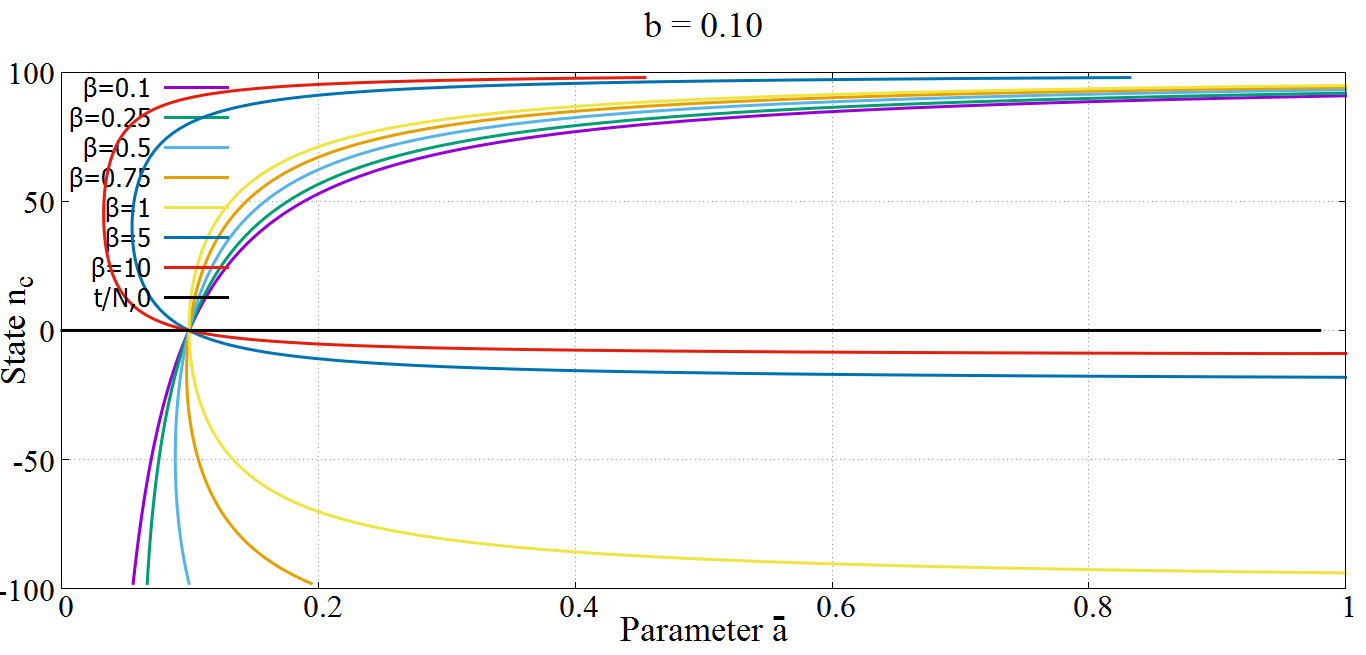
\includegraphics[width=\linewidth]{images/appendix/phaseSpace/1.png}
\end{figure}

\begin{figure}[h!]
 \centering
  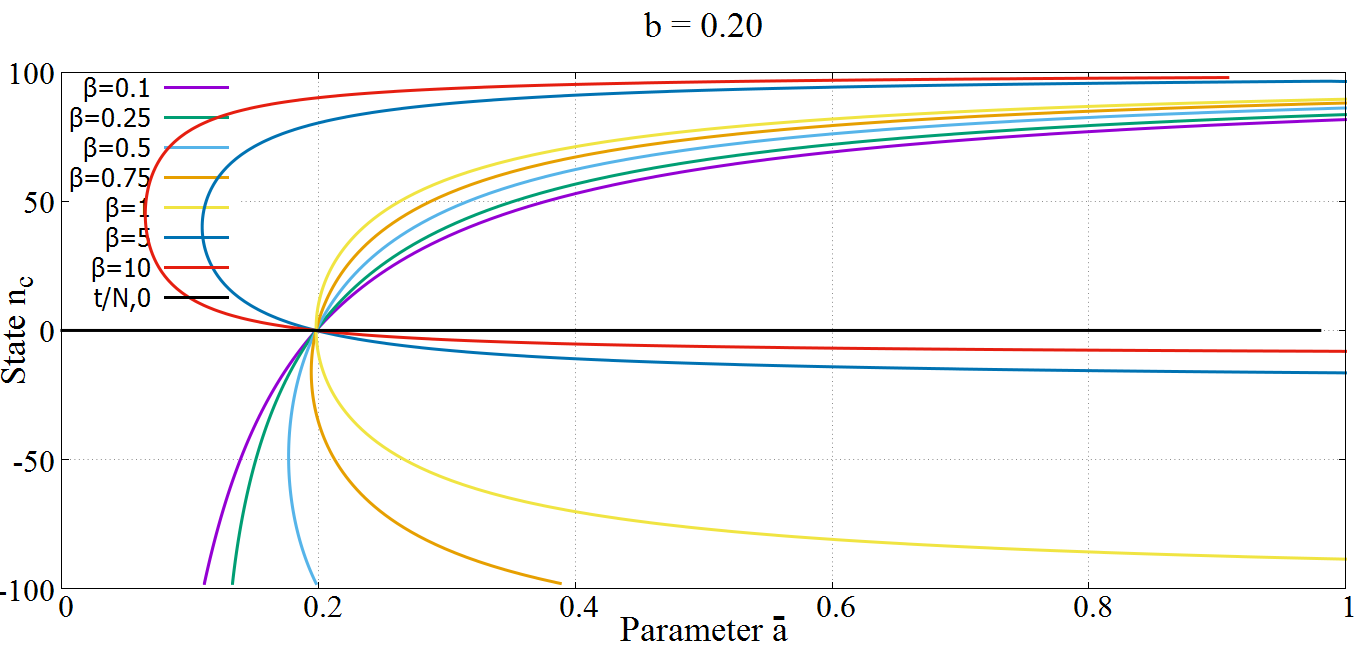
\includegraphics[width=\linewidth]{images/appendix/phaseSpace/2.png}
\end{figure}

\begin{figure}[h!]
 \centering
  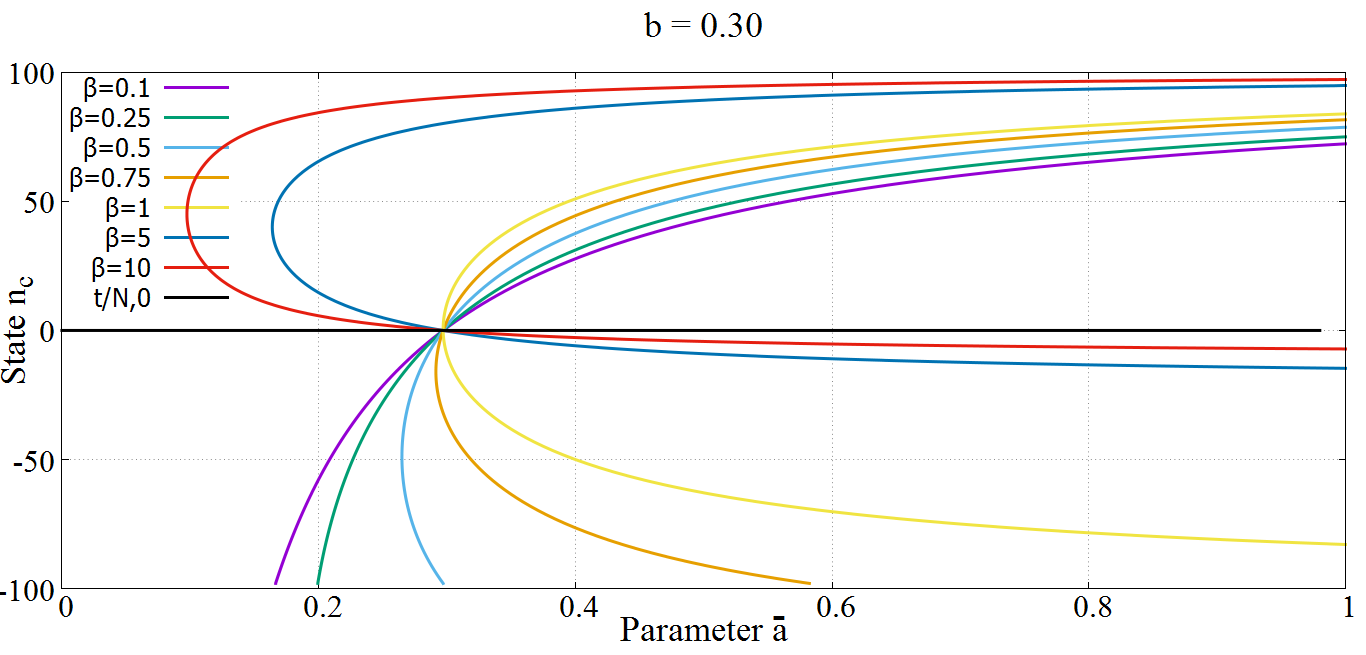
\includegraphics[width=\linewidth]{images/appendix/phaseSpace/3.png}
\end{figure}
\newpage
\begin{figure}[h!]
 \centering
  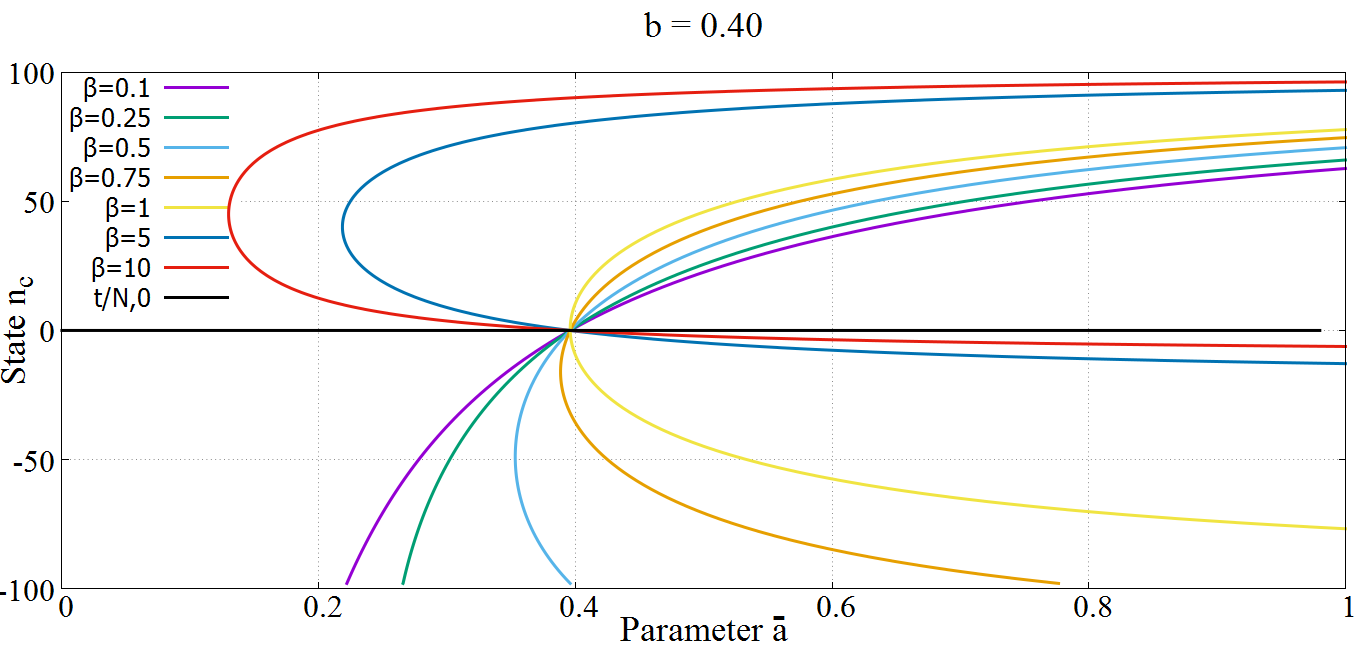
\includegraphics[width=\linewidth]{images/appendix/phaseSpace/4.png}
\end{figure}
\newpage
\begin{figure}[h!]
 \centering
  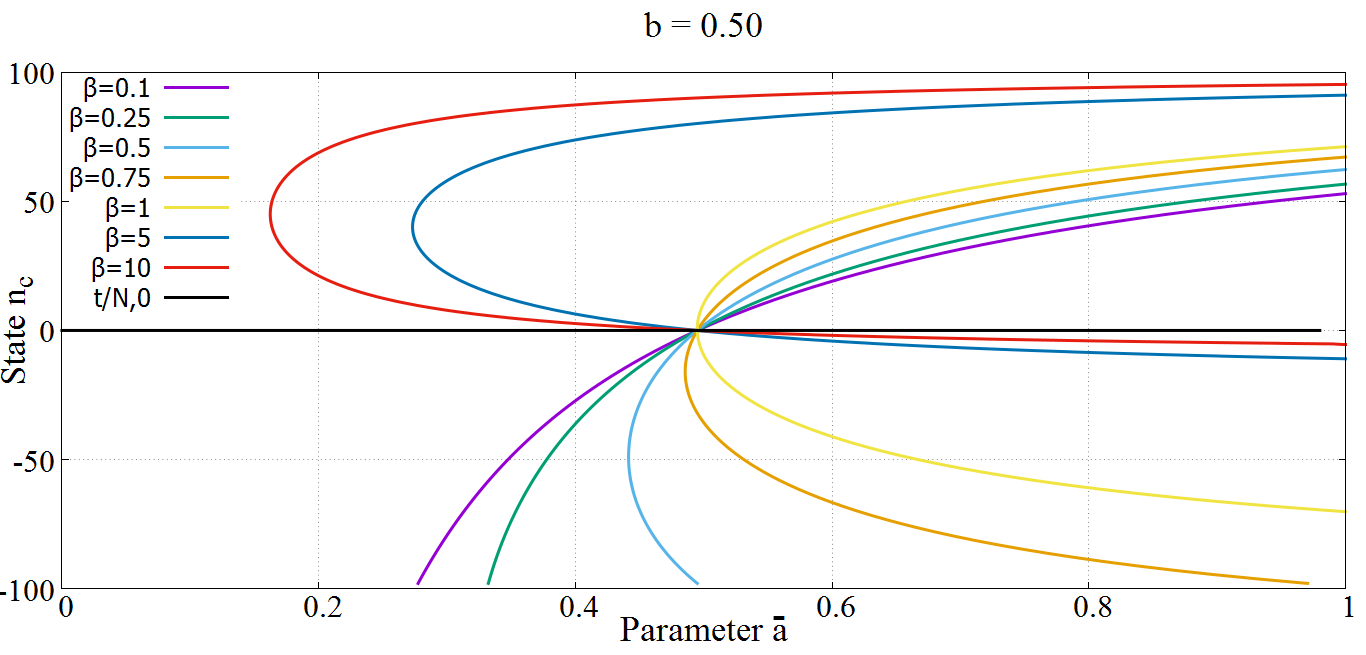
\includegraphics[width=\linewidth]{images/appendix/phaseSpace/5.png}
\end{figure}

\begin{figure}[h!]
 \centering
  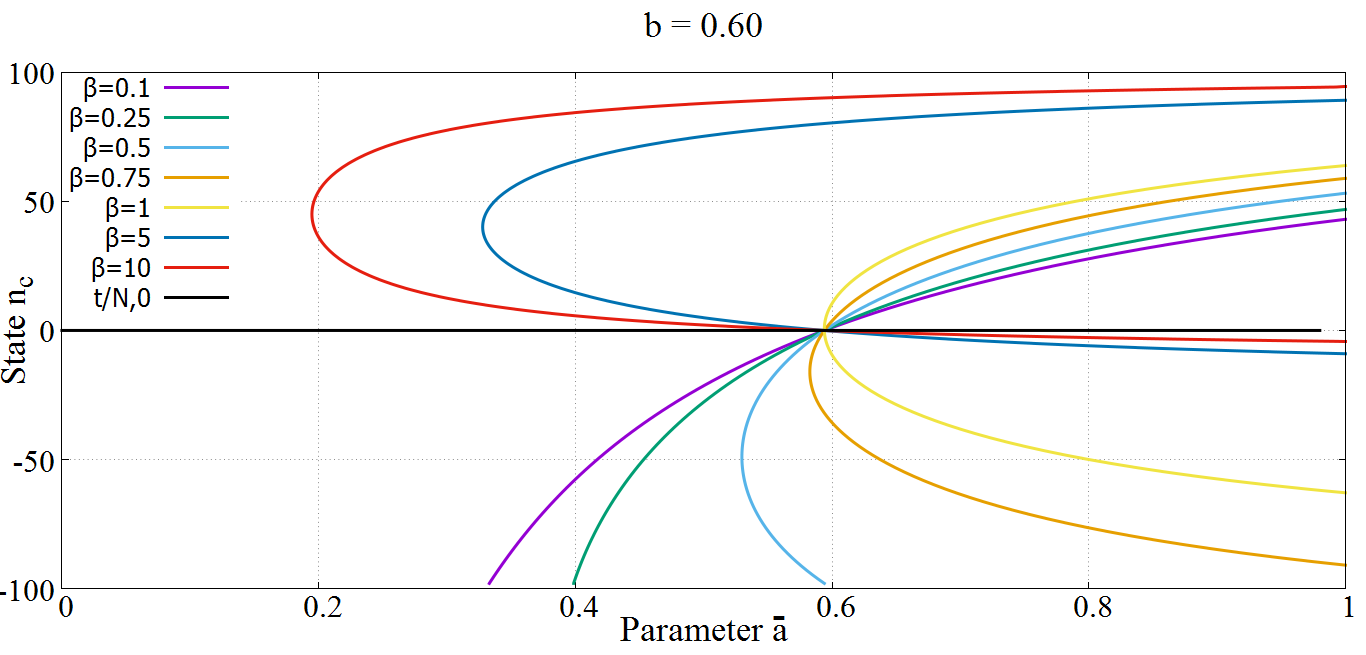
\includegraphics[width=\linewidth]{images/appendix/phaseSpace/6.png}
\end{figure}
\newpage
\begin{figure}[h!]
 \centering
  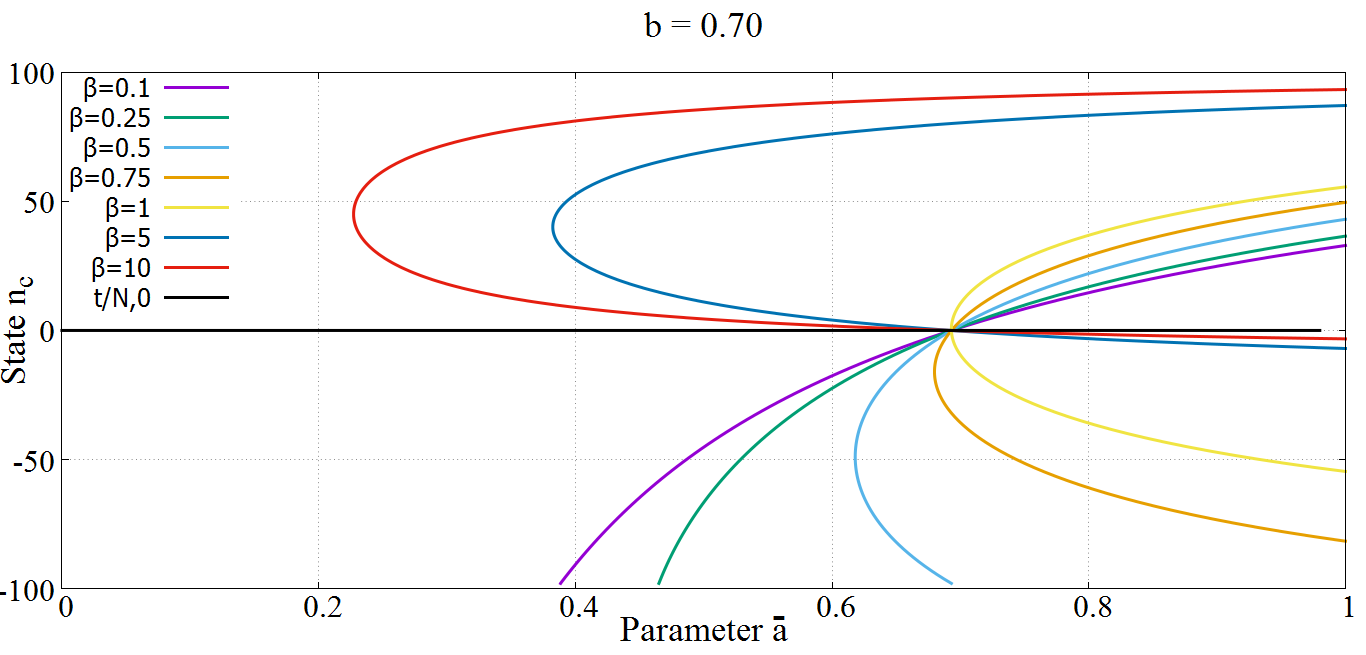
\includegraphics[width=\linewidth]{images/appendix/phaseSpace/7.png}
\end{figure}

\begin{figure}[h!]
 \centering
  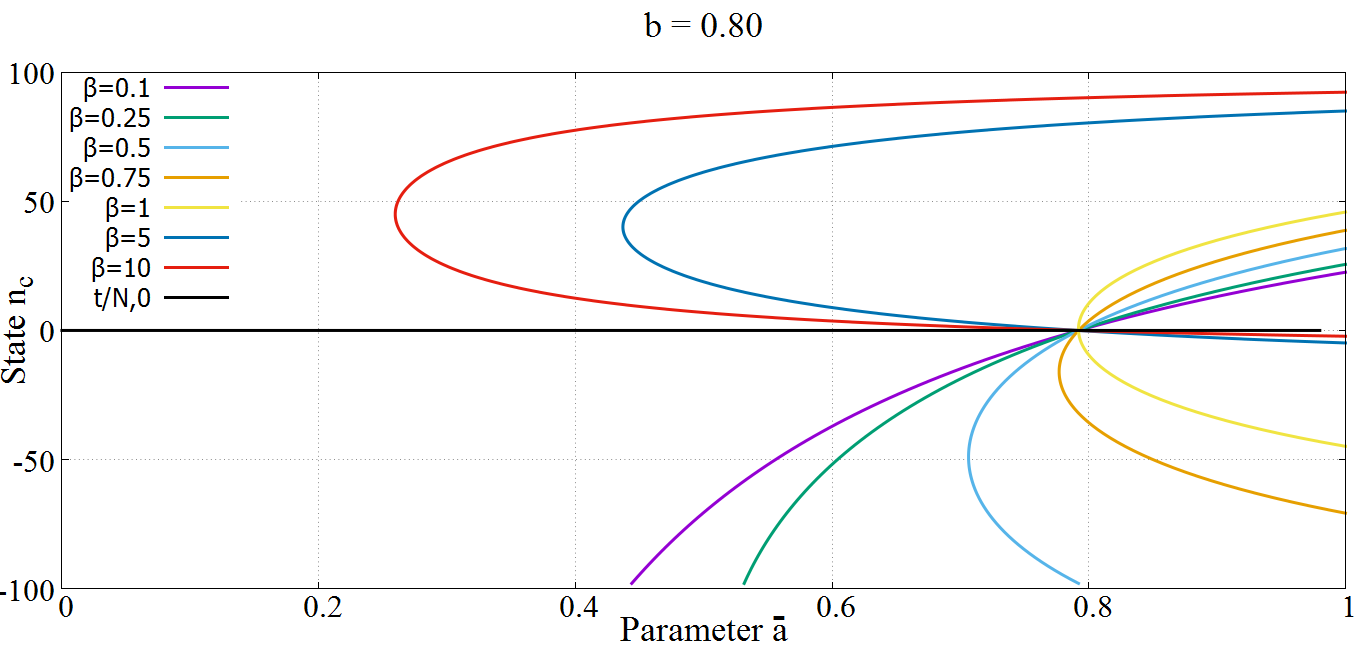
\includegraphics[width=\linewidth]{images/appendix/phaseSpace/8.png}
\end{figure}
\newpage
\begin{figure}[h!]
 \centering
  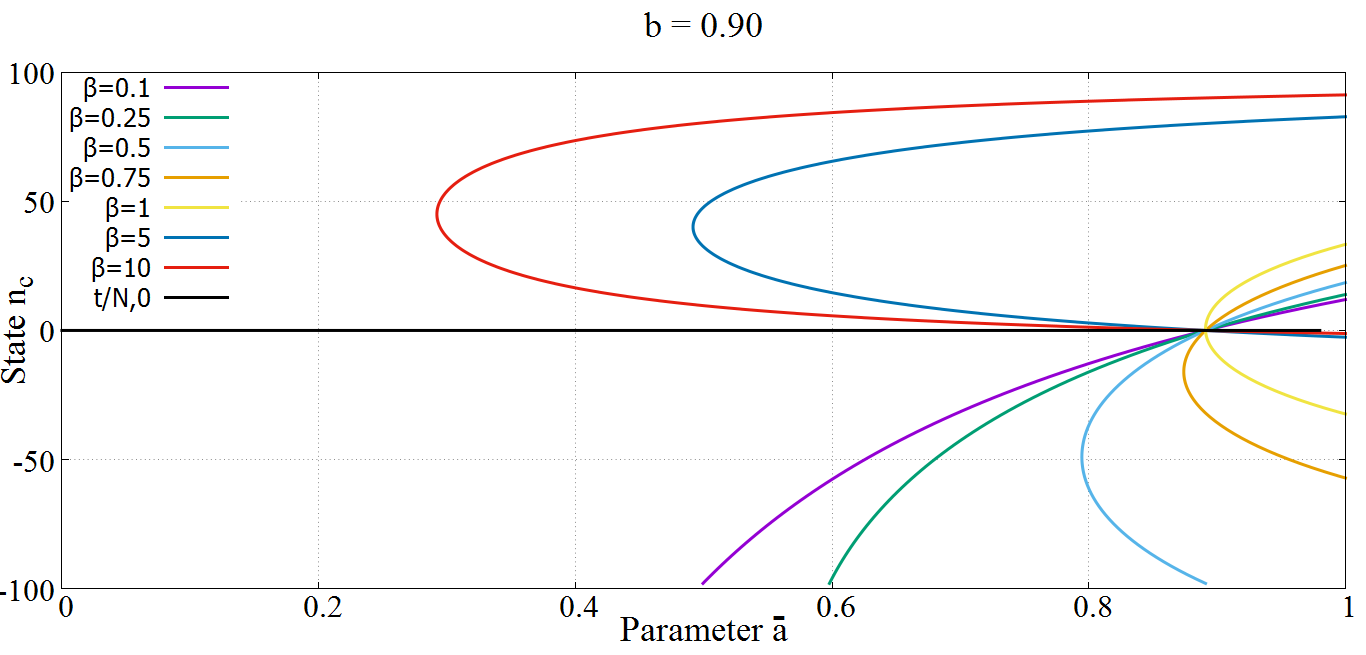
\includegraphics[width=\linewidth]{images/appendix/phaseSpace/9.png}
\end{figure}

\begin{figure}[h!]
 \centering
  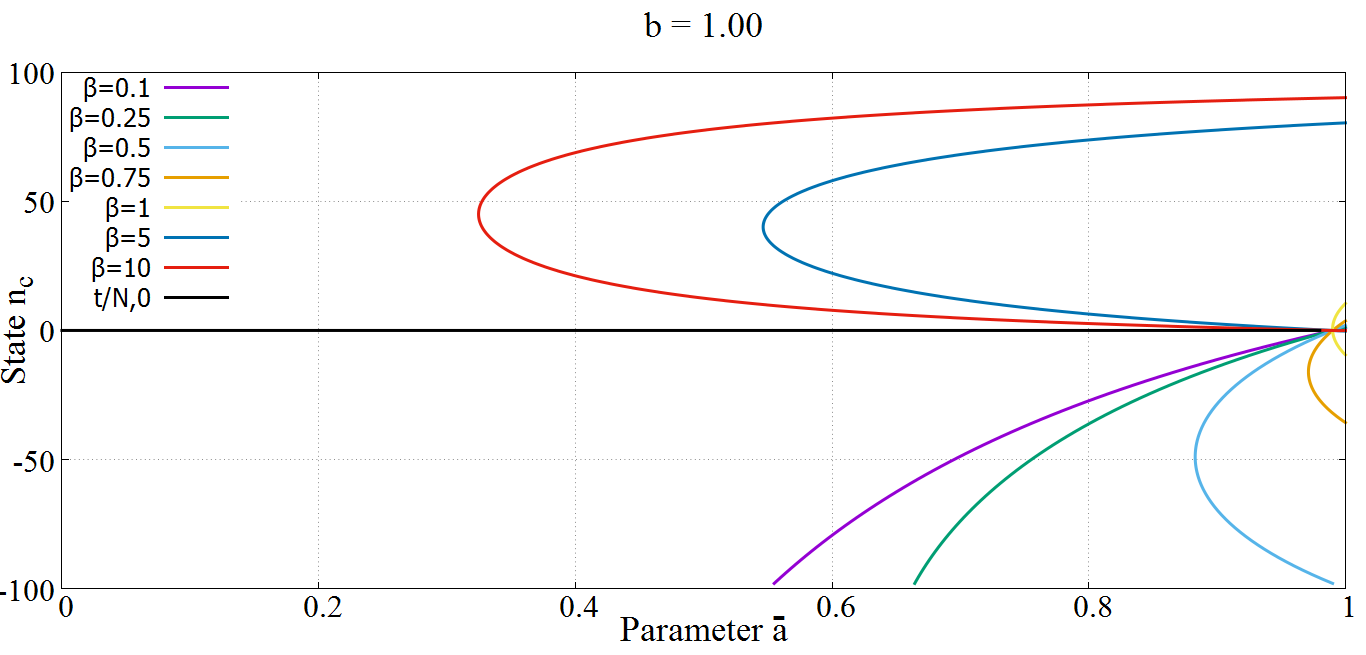
\includegraphics[width=\linewidth]{images/appendix/phaseSpace/10.png}
\end{figure}